\documentclass[a4paper]{article}

\usepackage{times}
\usepackage{tikz}
\usepackage[margin=0cm]{geometry}
\usepackage{graphicx}
\usepackage{anyfontsize}
\usepackage{fancyhdr}
\usepackage{indentfirst}
\usepackage{amsmath}
\usepackage[spanish]{babel}
\usepackage[utf8]{inputenc}
\usepackage{titlesec}
\usepackage{enumitem}
\usepackage{caption}
\usepackage{booktabs}

\author{}
\date{}
\title{}

\begin{document}
\thispagestyle{empty}

\newcommand{\saltoPag}{\newpage \noindent \thispagestyle{fancy}}

\begin{tikzpicture}[remember picture, overlay]
    \pgftransformshift{\pgfpoint{0cm}{0cm}}
    \draw [line width=2pt](1cm,-1cm) -- (1cm,-27.7cm) -- (14cm, -27.7cm) -- (14cm, -1cm) -- (1cm, -1cm);
    \draw[line width=2pt] (15cm, -27.7cm) -- (19cm,-27.7cm) -- (19cm, -1cm) -- (15cm, -1cm) --  (15cm, -27.7cm);
    \node [line width=2pt] at (17cm, -3.5cm) {
\includegraphics[width=3cm]{../../imagenes/utn.png}};
		\node [line width=2pt] at (7.5cm, -7.5cm) {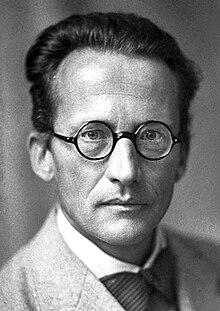
\includegraphics[width=6cm]{../../imagenes/schrodinger.jpeg}};
    \node at (17cm, -7cm) {\scalebox{5}{\textbf{U}}};
    \node at (17cm, -9cm) {\scalebox{5}{\textbf{T}}};
    \node at (17cm, -11cm) {\scalebox{5}{\textbf{N}}};
    \node at (17cm, -14cm) {\scalebox{5}{\textbf{F}}};
    \node at (17cm, -16cm) {\scalebox{5}{\textbf{R}}};
    \node at (17cm, -18cm) {\scalebox{5}{\textbf{C}}};
    \node at (7.4cm, -13cm) {\scalebox{2.5}{\textbf{Ecuación}}};
    \node at (7.4cm, -14cm) {\scalebox{2.5}{\textbf{de}}};
    \node at (7.4cm, -15cm) {\scalebox{2.5}{\textbf{Shrödinger}}};

    \node at (7.5cm, -22cm) {
        \begin{minipage}[c]{12cm}
            \begin{itemize}
                \raggedright
                \vspace{1.5cm}
                \item \fontsize{12}{12}\selectfont \textbf{Autores:} \vspace {1mm} \fontsize{11}{12}\selectfont \\
                    \begin{itemize}
                        \item \hspace{2mm} Valentino Rao - Leg. 402308 \\
                        \item \hspace{2mm} Ignacio Ismael Perea - Leg. 406265 \\
                        \item \hspace{2mm} Manuel Leon Parfait - Leg. 406599 \\ 
                        \item \hspace{2mm} Gonzalo Filsinger - Leg. 400460 \\ 
                        \item \hspace{2mm} Agustín Coronel - Leg. 402010 \\
                        \item \hspace{2mm} Santiago Pannunzio - Leg. 402350 \\
                        \item \hspace{2mm} Marcos Raúl Gatica - Leg. 402006 \\
                    \end{itemize}

                \item \fontsize{12}{12}\selectfont \textbf{Curso:} 2R1. \\
                \item \fontsize{12}{12}\selectfont \textbf{Asignatura:} Física electrónica. \\
                \item \fontsize{12}{12}\selectfont \textbf{Institución:} Universidad Tecnológica Nacional - Facultad Regional de Córdoba \\

            \end{itemize}
        \end{minipage}};

\end{tikzpicture}

\renewcommand{\normalsize}{\fontsize{12}{18}\selectfont}
\newgeometry{margin=1.75cm} %Quiero dejar esto cercano a las normas APA
\fancyhf{}
\renewcommand{\headrulewidth}{0pt}
\renewcommand{\footrulewidth}{0.4pt}
\fancyfoot[R]{[Rao V. - Parfait M. - Filsinger G. - Perea I. - Coronel A - Pannunzio S. - Gatica M.] [\textbf{pág. \thepage}]}
\setlength{\footskip}{0cm}
\newpage
\thispagestyle{empty}
\text{}

\titleformat{\section} {\fontsize{12}{12}\bfseries}{\thesection.}{0.5em}{\underline}

\newpage
\newpage

\thispagestyle{empty}
\setcounter{page}{0}
\tableofcontents

\saltoPag
\twocolumn
\flushbottom
\section{INTRODUCCIÓN}

    \subsection{Función de onda}
        \indent En la mecánica cuántica, la función de onda $\Psi$ describe el estado de una partícula en un sistema. Por si misma, $\Psi$ no tiene un significado físico directo, sin embargo, sirve para representar la densidad de probabilidad de encontrar una partícula en un lugar y momento dado (magnitud instantánea):

        \begin {center}
            $|\Psi|^2$
        \end{center}
        
        \indent Para una función de onda compleja, la densidad de probabilidad se calcula como:
        \begin{center}
            $|\Psi|^2 = (\Psi^*) (\Psi)$
        \end{center}

        Siendo $\Psi^*$ el complejo conjugado de $\Psi$. Lo que esta operación asegura que la densidad de probabilidad sea positivo y real (para que físicamente tenga significado).

        \indent La función de onda, $\Psi$, es una función compleja y se expresa:
    
        \begin{center}
            $\Psi = A + Bi$ \\
            $\Psi^* = A - Bi$ \hspace{5mm} \textit{(El complejo conjugado)} \\
        \end{center}

        Siendo A y B números reales.

        \indent Por lo tanto, una vez presentadas las funciones, es posible describir la densidad de onda compleja como:

        \begin{center}
            $|\Psi|^2 = (\Psi^*) (\Psi) = A^2 + B^2$
        \end{center}

    \subsection{La normalización}
        \indent Existen ciertas condiciones para que una función de onda represente de manera adecuada el estado de una partícula, siendo una de ellas que la densidad de probabilidad debe ser normalizable. \\
        \indent Normalizar $|\Psi|^2$ significa que debe ser integrable en todo el espacio y converger en un valor finito. Físicamente se puede interpretar que ese valor representa un lugar determinado en el espacio donde existe la partícula. La normalización es igual a:

        \begin{center}
            $\int_{- \infty}^{\infty} |\Psi|^2 dV = 1$ 
        \end{center}

        La ecuación hace referencia a la probabilidad total de encontrar la partícula en algún lugar del espacio equivale a 1. Si la función de onda compleja cumple la integral, cumple la normalización. También es posible multiplicar una constante a la función para cumplir a normalización en caso de no poder.

    \subsection{Funciones de onda ''bien comportadas''}
        \indent Para que una función de onda $\Psi$ sea válida en un sistema cuántico, debe:

        \begin{itemize} 
            \item Ser continua y de valor único en cada punto del espacio, ya que la probabilidad de encontrar una partícula en algún lugar específico debe ser un solo valor.
            \saltoPag
            \item Sus derivadas parciales, llámese:
                \begin{center}
                    $\frac {\partial \Psi}{\partial x}, \frac{\partial \Psi}{\partial y}, \frac{\partial \Psi}{\partial z}$
                \end{center}
            deben ser continuas y converger en un solo valor para cada punto en el espacio. Esto permite asegurar que no existan discontinuidades abruptas en la función de onda.
        \item $\Psi$ debe ser normalizable; tiende a 0 cuando $(x;y;z) \rightarrow \infty$.
        \end{itemize}

    \subsection{La interpretación probabilística}
        \indent Una vez aclarado las condiciones de normalización y de ''bien comportada'', la probabilidad de encontrar la partícula en una región específica del espacio puede calcularse integrando $|\Psi|^2$ en dicha región. \\
        \indent Supongamos que una partícula restringida a moverse en la dirección x, la probabilidad de encontrarla entre las posiciones $x_1$ y $x_2$ puede ser expresada por:

        \begin{center}
            $P(x_1 < x < x_2) = \int_{x_1}^{x_2} |\Psi|^2 dx $
        \end{center}

    \subsection{Contexto histórico y conceptual}
        \indent 
        


\end{document}
